
\newcommand{\vecc}[1]{\vec{\mathbf{#1}}}

\subsection{Overview and Domain Reduction}
% Overview
%   - we make a compiler
% for a restricted problem domain
% we generate a large amount of code
% we replace the lambda function with a call to this code
% pure functions with numerical input
% ignore the effects of numerical machine precision
Our solution will be a domain specific compiler that generates code for a conventional compiler e.g. g++ to optimise and turn into machine instructions.
We can define our goals for the compiler as follows:
\begin{itemize}
    \item Supports a large range of problems
    \item Generates code that is faster than the current default code
    \item Provides a user friendly interface for entering problems
    \item Practical to use (e.g. compile times are not too long)
\end{itemize}
To meet these goals it is first important to define the domain in which our compiler operates.

PDEs are mathematical functions.
Hence, we expect that all the substeps of solving PDEs are also mathematical functions.
This is certainly true in the FV scheme.
Looking at our main focus, the patch update step, we can say $\vecc{Q}_{out} = f(\vecc{Q}_{in}, t, dt, \vecc{x}, \vecc{dx})$ where
$\vecc{Q}_{in}$ and $\vecc{Q}_{out}$ are the input and output state of a patch,
$t$ is time,
$dt$ is the time step,
$\vecc{x}, \vecc{dx}$ are vectors describing the current patch's position and size, and $f$ is the patch update function.
Likewise, the numerical method and problem definitions can also be described as mathematical functions. 
Consequently, we can make the assertion that our compiler only needs to support pure functions.
This a useful restriction as it allows us to consider each function isolation, without the complication of side effects.

Our next observation is that mathematical functions accept a fixed length input and produce a fixed length output.
For example if $f$ is defined for $|\vecc{Q}_{in}|=100$ then the behaviour of $f$ on $|\vecc{Q}_{in}|=101$ is undefined.  
This eliminates the possibility of varying length inputs and outputs, again simplifying our compilers domain.
Further to this observation, every input and output is a real number.
We choose this to mean that all inputs and outputs are restricted to \texttt{double}.
This restriction could be relaxed to allow the use of all numerical data types e.g. \texttt{float}, \texttt{int} but will be left inplace to reduce the compiler complexity.

% mby somethingg about how x/3/3/3 == x/3^3

Finally we add the restriction that control flow is not supported.
At first this may appear to be too hash of a restriction which imposes a serious limit on the compilers capabilities.
However, as we will discuss in Section \ref{sec:DAG} a majority, if not all, control flow can be hoisted to DAG (Directed Acyclic Graph) creation as it is not a fundamental feature of the mathematical functions, hence this restriction is a non-issue.
An exception to this are peicewise functions e.g.
\[
    y = \begin{cases} g(x)  & \text{if } x<0.5 \\  h(x)  & \text{if } x\geq 0.5 \\\end{cases}
\]
This will not be supported by the compiler.





\subsection{DAG} \label{sec:DAG}
% What is a DAG - chip model
% [ ] Explain chip model
% [ ] Show example
% [ ] Control flow hoisting

Our compiler will begin with a Directed Acyclic Graph (DAG) as an input.
Currently it is the responsibility of a user to create such a DAG, however it would be entirely possible to generate a DAG using a user friendly format such as from a SymPy [REF] formula.
The DAG model we propose takes inspiration from hardware design and languages such a VDHL.

In a hardware design language you define electrical components.
Each component has input and output ports and its output is a function of its input.
Furthermore, it is common place to see specifications and test cases along side a component to be used in verification.

In our DAG every node has a set of input and output ports.
Every input port must receive single value and every output port can transmit copies of a single value.
Every node $n$ in our graph describes a function: $\vecc{out ports}=n(\vecc{in ports})$ with the number of inputs and outputs being of a fixed length.

A node may be primitive and directly map to a primitive code operation, for example an addition node maps to $out_1 = in_1 + in_2$ (see Figure \ref{fig:bin_add}).
Or a node may be composite, where it is a DAG itself.
Composite nodes would map to functions in the final code output.
Figure \ref{fig:bn} demonstrates composite nodes with the calculation $out_0 = (in_0)^3 + in_1$ where the function \textit{cubed} has been implemented as a subgraph.
The nested structure that composite nodes create provides a lot of expressive power.
For example, a user can create Problem Definition DAGs, then hand those DAGs to pre-made Patch Update and Numerical Ingredient DAG builders to create a DAG that describes the full Patch Update process.


\begin{figure}[h!]
    \begin{center}
        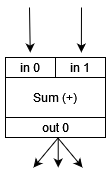
\includegraphics[width=.15\textwidth]{binary_add.png}
        \caption{Example of binary addition as a DAG node.}
        \label{fig:bin_add}
    \end{center}
\end{figure}

\begin{figure}[h!]
    \centering
    \subcaptionbox{Top level\label{fig:bn1}}{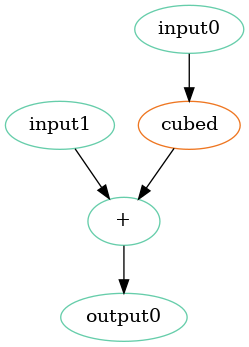
\includegraphics[width=.2\textwidth]{basic-nested-part1.png}}
    \hspace{1em}
    \subcaptionbox{Exploded view\label{fig:bn0}}{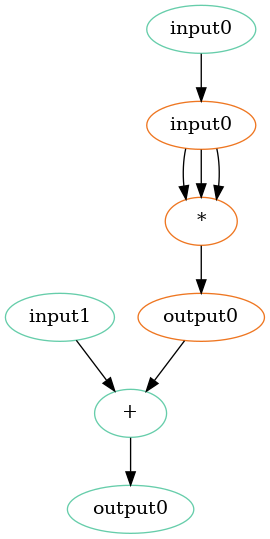
\includegraphics[width=.2\textwidth]{basic-nested-part0.png}}
    \caption{Example of a nested DAG that calculates $out_0 = (in_0)^3 + in_1$. NOTE the visualisation displays a node's input edges in a random order.}\label{fig:bn}
\end{figure}

Provided that the graph is acyclic we can always find an order to evaluate every node in the graph for some given input.
In our compiler every DAG node implements an \texttt{eval} function which takes its inputs as a list and returns the outputs as a list.
The \texttt{eval} function allows us to test every DAG we define using unit and integration tests.

DAGs are created in python.
Every node type is a class.
To create a node you create an object from the class of node you desire.
Graph nodes are a special class of Node that implement additional functions.
Namely, graph nodes store a sparse definition of the graph they represent and provide an interface for users to add edges to the graph.
The \texttt{eval} functions of all the primitive nodes are simple, often only preforming one operation.
The \texttt{eval} function for a DAG node is more complex, first calculating a valid traversal order of the DAG.
Then following this traversal order, the DAG node calls the \texttt{eval} function on each subnode, forwarding the output of completed \texttt{eval} to the input of nodes yet to be processed.
This process repeats until the entire DAG has been traversed.

Using python to create DAGs allows for the hoisting of control flow.
For example, take the a flux function used in an ExaHyPE project:
\begin{lstlisting}[language=c]
void flux(
  const double * __restrict__ Q, // input
  ...
  int normal,
  double * __restrict__ F // output
)  {
  switch(normal){  
  case 0: //in x direction
	  F = flux_x(Q, ...)
	  break;
  case 1: //in y direction
	  F = flux_y(Q, ...)
	  break;
  }  
}
\end{lstlisting}
The switch control flow is run every evaluation of flux and depends on the value of the normal.
However, in Patch Update the value the normal is known at compile time.
Therefore, we can use a builder patten in python to hoist this control flow out of the flux function.
\begin{lstlisting}[language=python]
def build_flux_DAG(normal:int)->DAG:
    if normal==0:
        return build_flux_x()
    else:
        return build_flux_y()
\end{lstlisting}




\subsection{IR}
% What is the IR - llvm inspired
% [ ] Explain IR
% [ ] Show example


DAGs are an powerful and expressive way to represent an input problem, however code generation directly from a DAG is challenging.
To overcome this issue we introduce an intermediate representation (IR).
The goal of this IR is to offer a middle ground between the DAG and output code.
It should be easy to transform the DAG into an IR, and it should be easy to transform this IR into code.
The IR we use takes inspiration from llvm.
It is a set of function definitions, and within each function definition there is a linear sequence of instructions.

One of the main challenges we came across during the code generation process was variable management.
Our compiler supports interchangeable code generation backends, allowing different languages to be targeted.
This means it's preferable to include information such as variable declaration and complex function signatures in the IR, allowing code generation backends to stay as slim as possible.
However, the complications induced by variable declarations and function signatures are a key reason why code generation directly from a DAG is hard.   


To combat these opposing requirements we create 2 standards for our IR.
The IR can be loose, and the IR can be tight.
When we transform our DAG we transform it into a loose IR.
A loose IR doesn't worry about variable declaration, variable declaration is implicit like in python.
There are also useful tools available in loose IRs such as a special class of temporary variables.
Finally, loose function signatures are kept very simple.
A loose function maintains a list of (possibility hundreds) of single value input variables and a list of (possibly hundreds) of single value output variables.
The relaxed nature of the loose IR makes it ideal for preforming transforms (such as for optimisations) as there are few ways to invalidate a loose IR.
On the other hand, a tight IR is much stricter.
In a tight IR all variable must be named and declared.
And a tight function signature mirrors that of the target output code, containing a mixture of input and output variable that can be single values or arrays.

\begin{figure}[]
\begin{tabular}{rl}
     \multirow{2}{*}{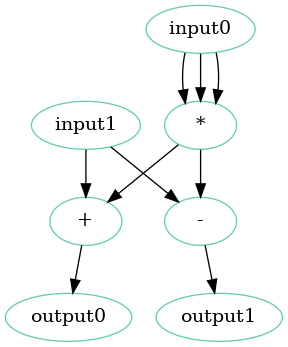
\includegraphics[width=0.2\textwidth]{tight_vs_loose.png}}&
    \begin{lstlisting}[language=c]
define IR_DataTypes.VOID @kernel (%in0, %in1) (%out0, %out1):
	%tmp1 = %in0
	%tmp2 = %tmp1 * %tmp1 * %tmp1
	%tmp3 = %in1
	%tmp4 = %tmp2 + %tmp3
	%tmp5 = %tmp4
	%tmp6 = %tmp2 - %tmp3
	%tmp7 = %tmp6
	%out0 = %tmp5
	%out1 = %tmp7
\end{lstlisting}\\
    & \begin{lstlisting}[language=c]
define IR_DataTypes.VOID @kernel (new #list(in), new #list(out)):
	new #tmp2 = #in[0] * #in[0] * #in[0]
	#out[0] = #tmp2 + #in[1]
	#out[1] = #tmp2 - #in[1]
	<return nothing>
\end{lstlisting} \\
\end{tabular}
\caption[My beautiful figure.]{\label{fig:label}My beautiful figure}
\end{figure}


\newsavebox{\firstlisting}
\begin{lrbox}{\firstlisting}% Store first listing
\minipage{.33\textwidth}
\begin{lstlisting}
define IR_DataTypes.VOID @kernel (%in0, %in1) (%out0, %out1):
	%tmp1 = %in0
	%tmp2 = %tmp1 * %tmp1 * %tmp1
	%tmp3 = %in1
	%tmp4 = %tmp2 + %tmp3
	%tmp5 = %tmp4
	%tmp6 = %tmp2 - %tmp3
	%tmp7 = %tmp6
	%out0 = %tmp5
	%out1 = %tmp7
\end{lstlisting}
\endminipage
\end{lrbox}

\newsavebox{\secondlisting}
\begin{lrbox}{\secondlisting}% Store first listing
    
\minipage[t]{.33\textwidth}
\begin{lstlisting}
define IR_DataTypes.VOID @kernel (new #list(in), new #list(out)):
	new #tmp2 = #in[0] * #in[0] * #in[0]
	#out[0] = #tmp2 + #in[1]
	#out[1] = #tmp2 - #in[1]
	<return nothing>
\end{lstlisting}
\endminipage
\end{lrbox}

\begin{figure}
\centering

\sbox{\measurebox}{%
  \begin{minipage}[b]{.33\textwidth} \centering
        \fbox{\subfloat[]{\label{fig:figB}\fbox{\usebox{\firstlisting}}}}
        \subfloat[]{\label{fig:figC}\usebox{\secondlisting}}
  \end{minipage}
}

\usebox{\measurebox}\qquad
    \begin{minipage}[b][\ht\measurebox][s]{.33\textwidth}
      \fbox{\subfloat[]{\label{fig:figA}\fbox{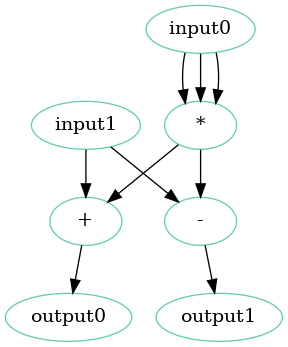
\includegraphics[width=\textwidth]{tight_vs_loose.png}}}}
       
    \end{minipage}
\caption{my caption. (a) is .... (b) is .... (c) is ....}
\label{fig:Test}
\end{figure}


\minipage[b][\ht\measurebox][s]{.33\textwidth}
\begin{lstlisting}[language=c]
define IR_DataTypes.VOID @kernel (new #list(in), new #list(out)):
	new #tmp2 = #in[0] * #in[0] * #in[0]
	#out[0] = #tmp2 + #in[1]
	#out[1] = #tmp2 - #in[1]
	<return nothing>
\end{lstlisting}
\endminipage


\subsection{Compiler Architecture}
Our compiler consists of 3 stages.
The DAG transform stage, the IR transform stage, and the code generation stage.

% DAG Transforms
In the DAG transform stage a series of user specified transforms are applied to the DAG.
The most useful of these transforms is the flatten transform.
% FIG?
This transform takes a nested DAG (i.e. a DAG containing composite nodes) and for every composite node, the composite node is deleted and replaced by a copy of the DAG contained within the composite node.
Applied recursively, a highly nested DAG can be reduced to only contain primitive nodes, i.e. it is flattened.
This transform causes the final output code to be a single monolithic function, as opposed to a function containing many function calls.
Another notable transform we investigated was the removal of duplicated computation.
Within a DAG, duplicate computation manifests itself as 2 equivalent nodes (e.g. 2 addition nodes) that share the same inputs.
Once 2 such nodes are identified one can be deleted, and its output edges copied over to the node that remains.
Some care has to be taken if an operations is commutative (e.g. addition and max) or not (e.g. subtraction and division).

% DAG -> IR
Once all the user DAG transforms are completed the DAG is transformed into the IR.
To do so, the DAG and every sub-DAG are identified and processed separately to create a set of loose functions.
When processing a DAG we create a valid traversal order, much like DAG \texttt{eval} does.
Then following this order, every node in the DAG is transformed into an IR symbol.
Primitive nodes map to equivalent primitive IR Symbols and composite nodes map to loose IR function calls.
The output of every port of every node is stored as a new temporary variable, and these temporary variables are passed as the input to other nodes.
At the end of the transform we have an IR in loose form.

% IR Transforms 
The second stage of the compiler is the IR transform stage.
Much like we apply a series of user defined DAG transforms, so to do we apply a series of user defined IR transforms.
Interestingly there are equivalences between DAG transforms and IR transforms.
For example, the DAG transform \texttt{Remove Passthrough Nodes}, which removes all the primitive nodes that simply pass through a single value, is approximately equivalent to the IR transform \texttt{Remove Forward Aliasing}, which removes all lines that look like \lstinline{%tmp_x=%tmp_y} (i.e. a line that copies a single value).
However, it is not the case that all IR and DAG transforms share this equivalence.
For example, in the IR you can create transforms to arrange a programs memory layout, but in a DAG there is no concept of memory layout.

% Loose IR -> Tight IR
%   - variable model
%   - function stencil 
Once the user defined IR transforms are applied the IR is transformed into a its tight form.
This process begins by applying user defined function signatures to loose IR functions, these are called function stencils.
This transforms all loose functions and function calls into tight functions.
A function function stencil consists of 3 parts: the desired arrangement of arguments in the tight function; a map from input variable to variable in the function argument; and a map of output variable to function arguments.

Once function stencil are applied, every temporary variable is replaced with a named variable.
A named variable is any variable that has a unique name and can be generated into code e.g. a normal variable and an array element.
The distinction between temporary variables and named variables may seem like unnecessary bloat, however it does serve an important propose.
Users may choice to create transforms that arrange their programs memory layout, for example targeting a SIMD friendly layout.
To do so they will replace temporary variables with named variables.
As it is not expected that users will tackle memory layout this transform creates a new normal variable for every temporary variable. 

The finally all the named variables are defined, creating a tight IR.
For the most part this involves defining a variable the first time it is observed.
However, special care is required for variables that are defined in the function signature and also for elements of arrays.

% Tight IR -> Code
The final step of the compiler is to transform the tight IR into code.
The compiler supports interchangeable code generation backends (CGB), however we have only implemented a C++ backend.
Within the C++ CGB we use the cparser python package.
The cparser package defines AST nodes (Abstract Syntax Tree) for C, and given an AST can generate code.
This reduces the problem of code generation to a problem of transpilation from the IR AST to a C AST.
This can be achieved with a post order traversal of the IR AST, generating C AST nodes from each of the IR AST nodes.
Finally, some post processing is preformed to transform the C into C++.
For example, the required standard library headers are inserted, and variable decorators such as \lstinline{__restrict__} are added.  